\documentclass[a4paper]{article}
\usepackage{fontspec}
\setmainfont{Linux Libertine O}[Scale=MatchLowercase]
\usepackage{xeCJK}
\setCJKmainfont{NotoSansCJK-Regular.ttc}[
	Path = /usr/share/fonts/noto/,
]
% \usepackage[absolute,noshowtext,showboxes]{textpos}
\usepackage[absolute,showboxes]{textpos}
% \textblockorigin{-0.02cm}{0.07cm} %HPDeskJet5160
% \textblockorigin{0.00cm}{0.00cm} %HPDeskJet5160
\textblockorigin{0.00cm}{0.00cm} %HPDeskJet5160
% \textblockorigin{0.05cm}{0.13cm} %HPDeskJet5160
% \textblockorigin{0.00cm}{0.00cm} %HPLaserJet5000LE
\usepackage{graphicx}
\graphicspath{ {/home/$ENV{USER}/ttb/trunk/forms/bean/} }
\pagestyle{empty}
\setlength{\unitlength}{1cm}

\setlength{\TPVertModule}{2.1214cm}

\newcommand{\myXseventeenBeanXIdentifier}[0]{
seventeen bean
}

\newcommand{\myXseventeenBean}[0]{
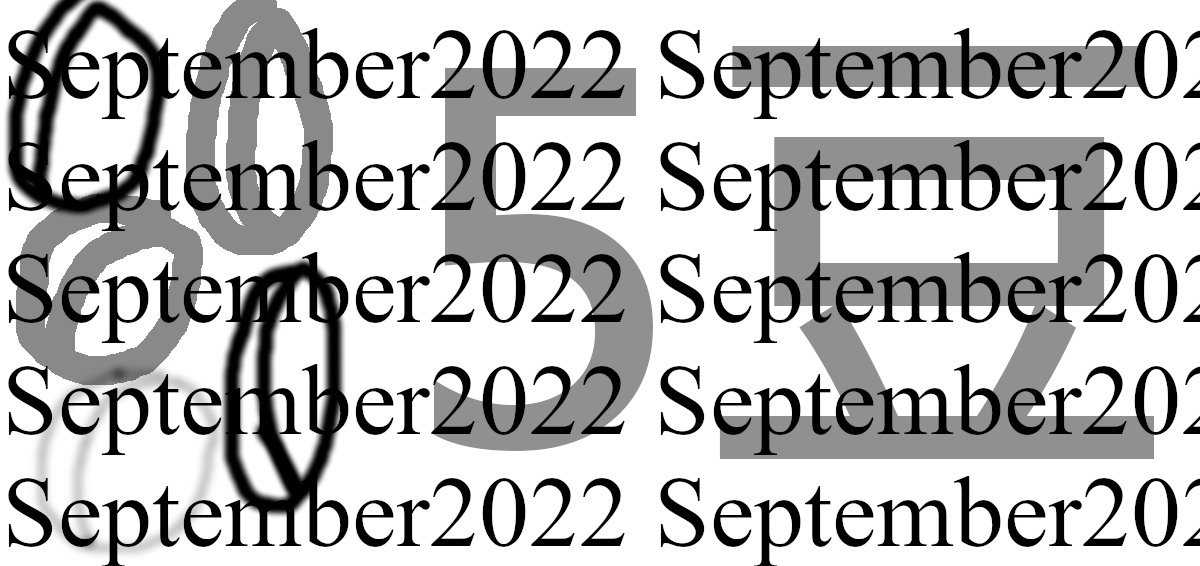
\includegraphics[angle=00,height=0.057\paperheight,width=0.150\paperwidth]{seventeen_bean.png}
}

\newcommand{\myXsixteenBean}[0]{
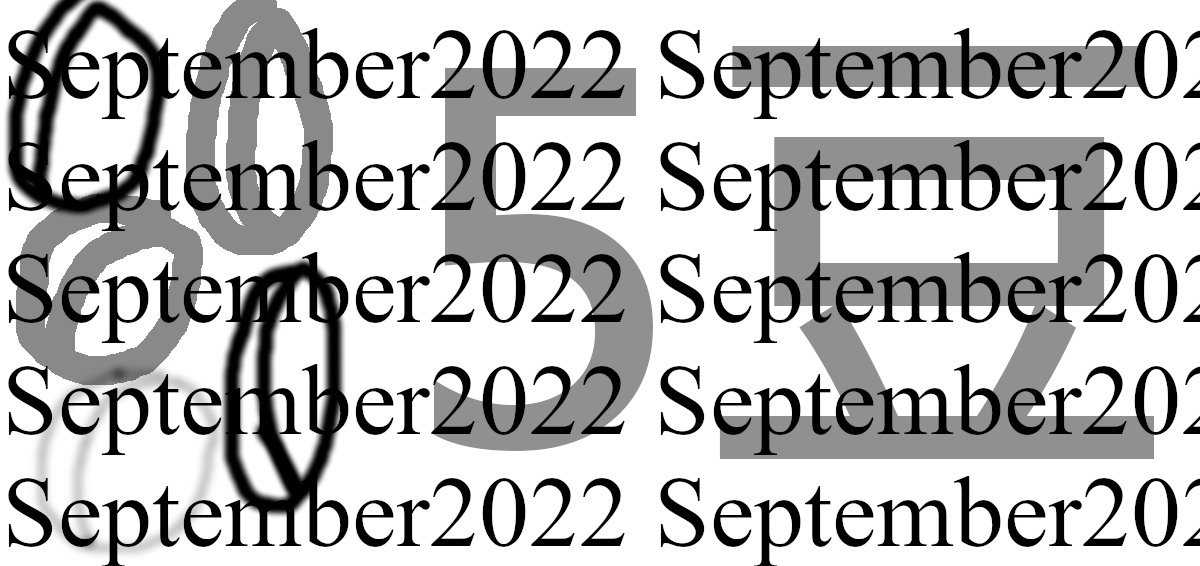
\includegraphics[angle=00,height=0.057\paperheight,width=0.150\paperwidth]{sixteen_bean.png}
}

\newcommand{\myXfourteenBean}[0]{
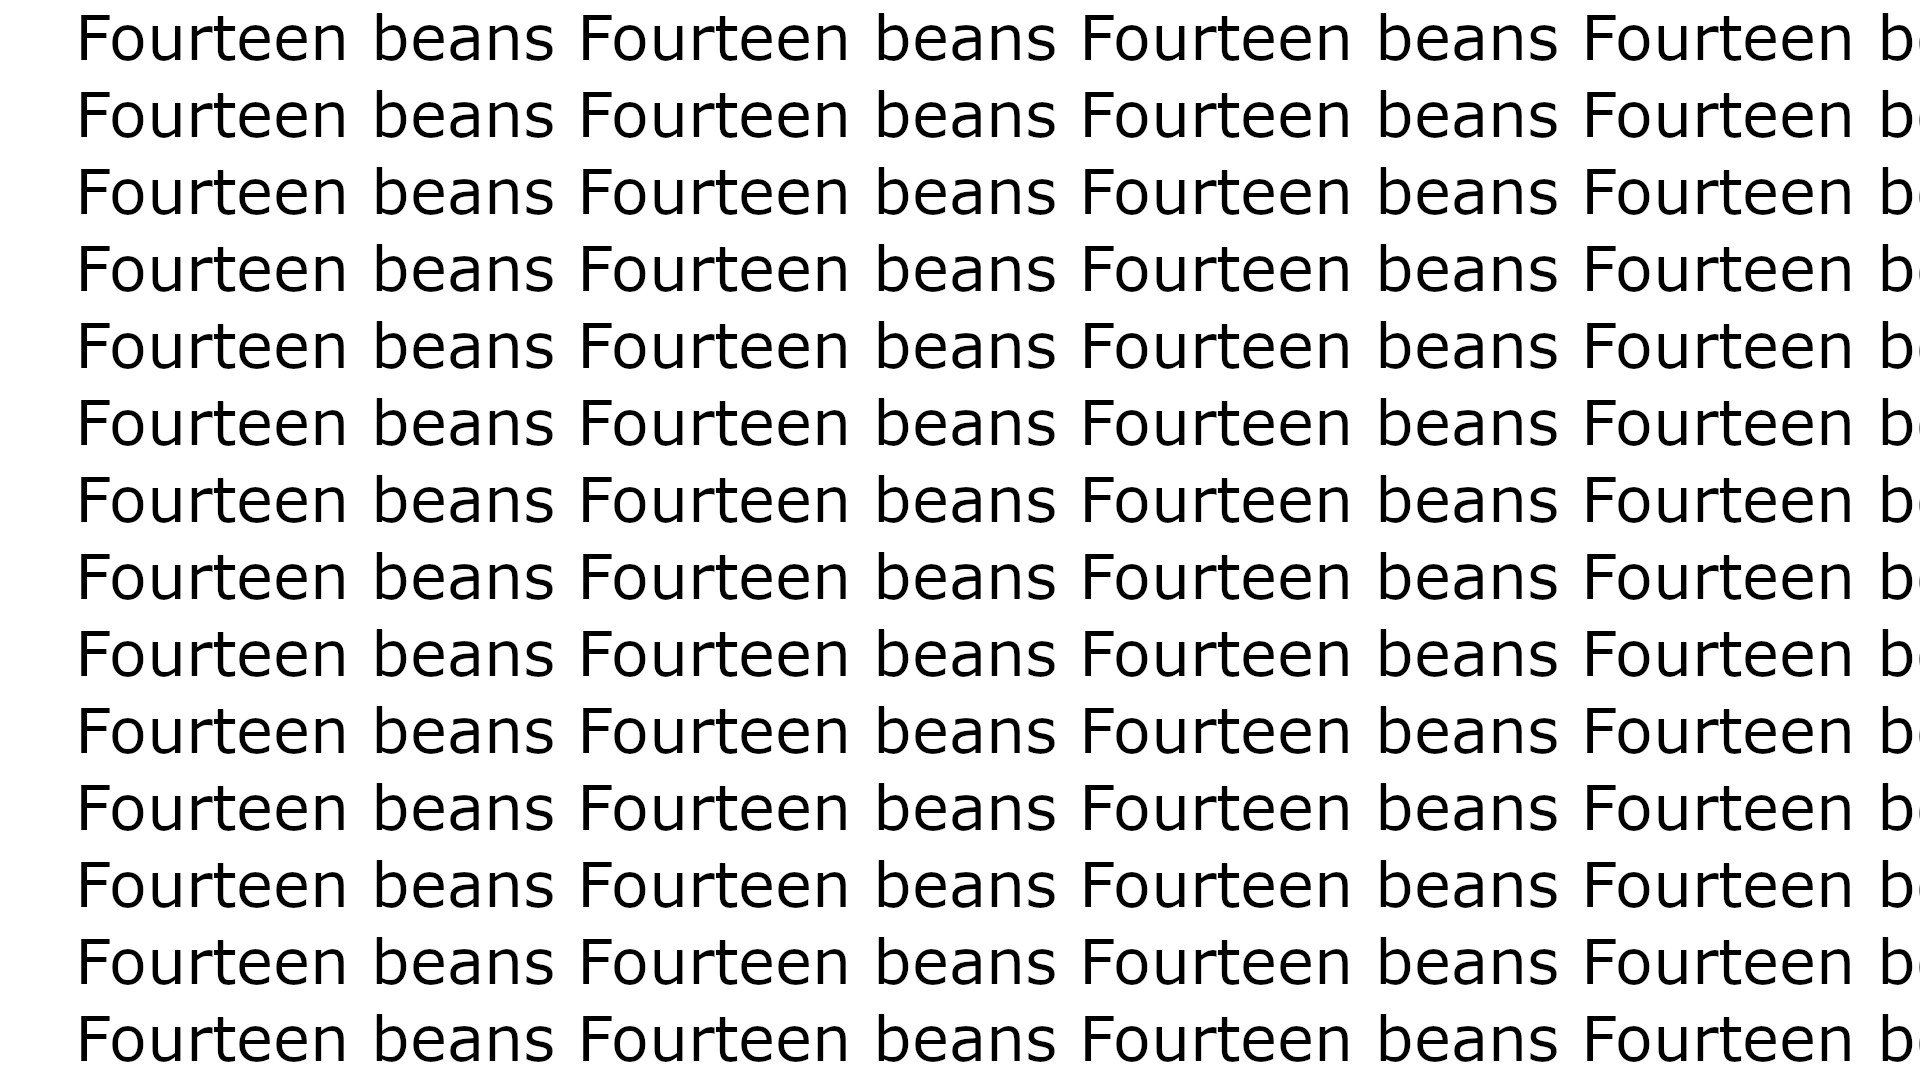
\includegraphics[angle=00,height=0.057\paperheight,width=0.150\paperwidth]{fourteen_bean.png}
}

\newcommand{\myXthirteenBean}[0]{
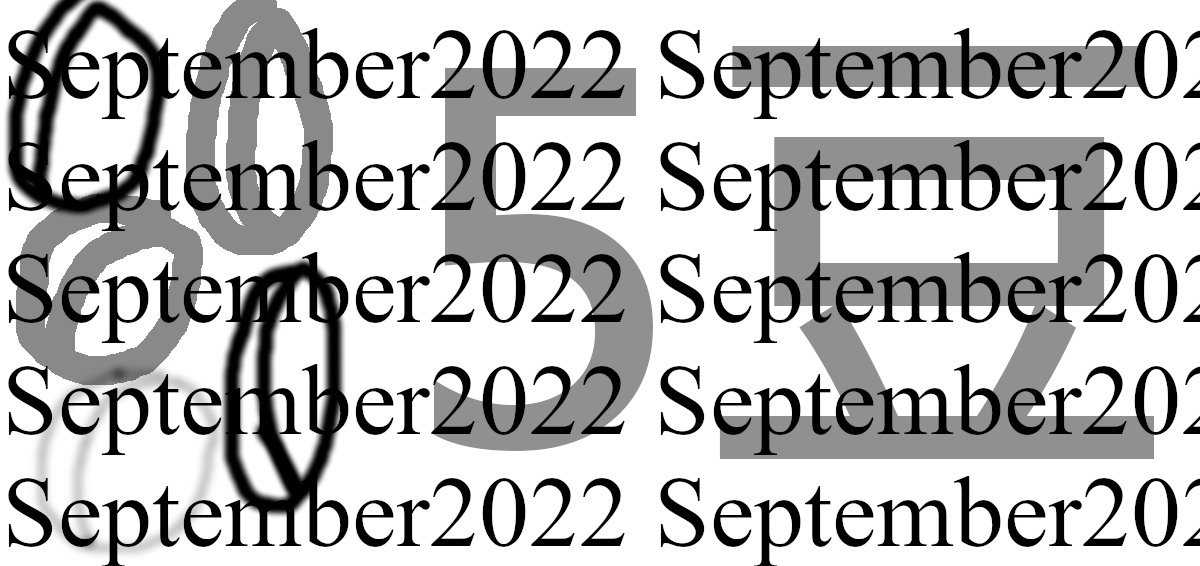
\includegraphics[angle=00,height=0.057\paperheight,width=0.150\paperwidth]{thirteen_bean.png}
}

\newcommand{\myXelevenBean}[0]{
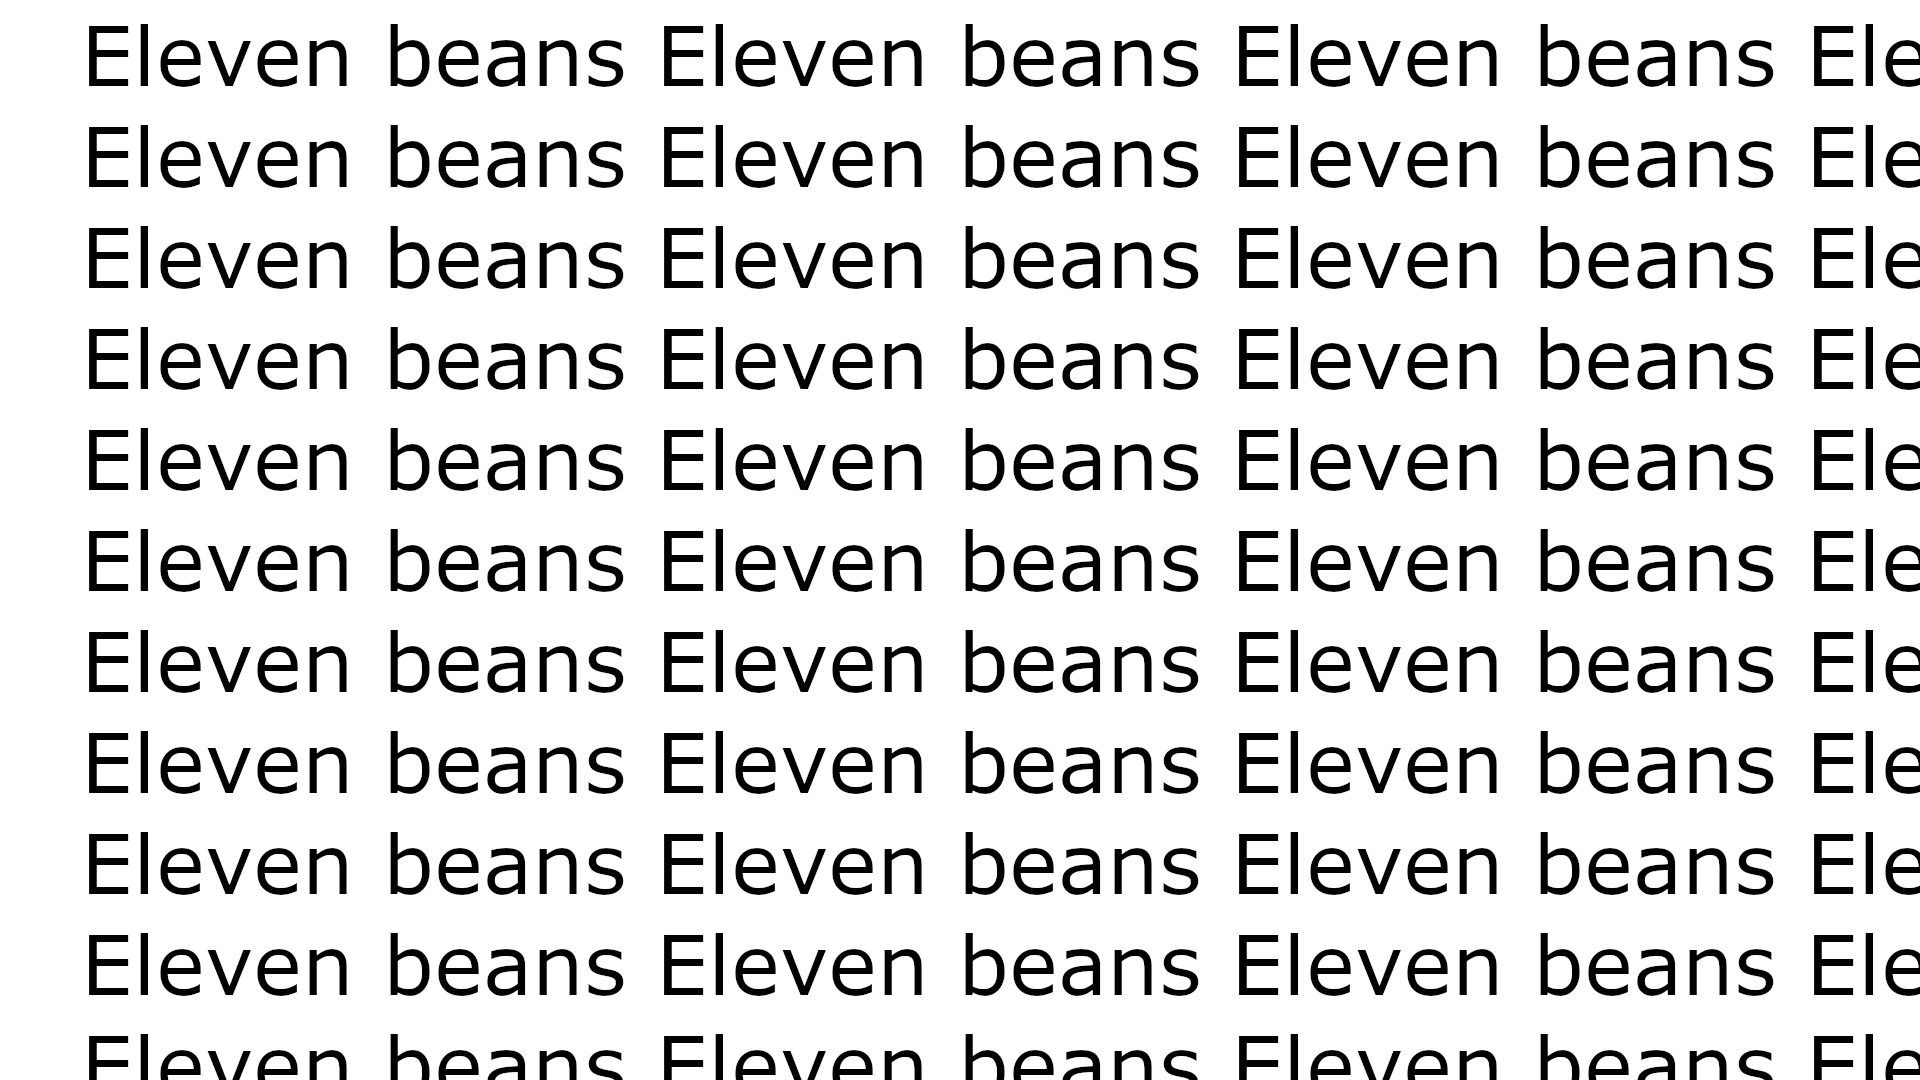
\includegraphics[angle=00,height=0.057\paperheight,width=0.150\paperwidth]{eleven_bean.png}
}

\newcommand{\myXtenBean}[0]{
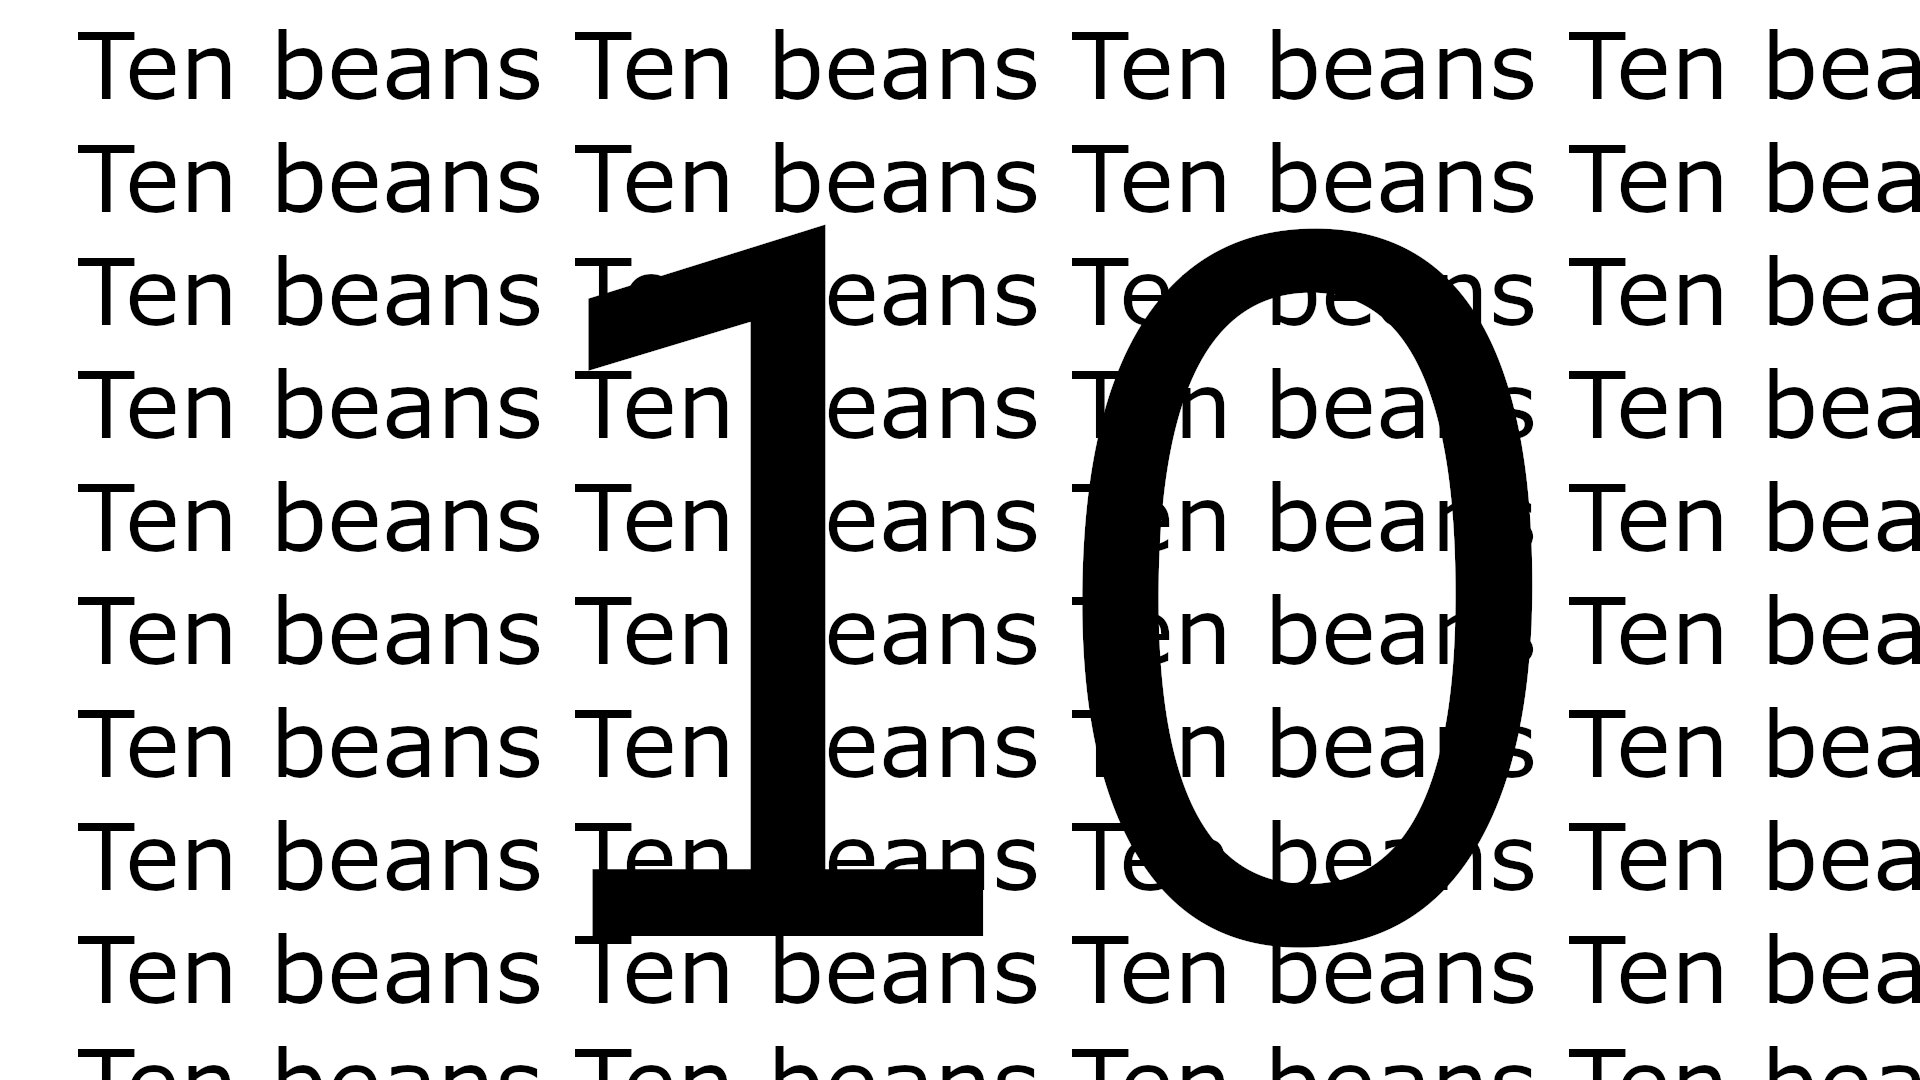
\includegraphics[angle=00,height=0.057\paperheight,width=0.150\paperwidth]{ten_bean.png}
}

% \newcommand{\myDcontent}[0]{
% 
% }

\newcommand{\mycard}[5]{%
	\vspace{0.35cm}
	\tiny #1 #2
	% \vspace{-0.03cm}
	% \par
	\parbox[t][0.058\paperheight][c]{0.150\paperwidth}{%
	\hspace{-0.65cm} \large#3\\
	}
}

\begin{document}
% \begin{picture}(15,20)(+4.8,-22.05)
% \begin{tabular}[t]{*{2}{|p{10.05cm}}|}

% top line

\begin{textblock}{2.67}(0,0)
\textblocklabel{picture1}
\mycard{}{}{
\myXseventeenBean
}{}{} 
\end{textblock}

\begin{textblock}{2.67}(2.67,0)
\textblocklabel{picture2}
\mycard{}{}{
\myXsixteenBean
}{}{} 
\end{textblock}

\begin{textblock}{2.67}(5.33,0)
\textblocklabel{picture1}
\mycard{}{}{
\myXfourteenBean
}{}{} 
\end{textblock}

\begin{textblock}{2.67}(8.0,0)
\textblocklabel{picture2}
\mycard{}{}{
\myXthirteenBean
}{}{} 
\end{textblock}

\begin{textblock}{2.67}(10.67,0)
\textblocklabel{picture3}
\mycard{}{}{
\myXelevenBean
}{}{} 
\end{textblock}

\begin{textblock}{2.67}(13.33,0)
\textblocklabel{picture5}
\mycard{}{}{
\myXtenBean
}{}{} 
\end{textblock}

% second line

\begin{textblock}{2.67}(0,1)
\textblocklabel{picture1}
\mycard{}{}{
\myXseventeenBean
}{}{} 
\end{textblock}

\begin{textblock}{2.67}(2.67,1)
\textblocklabel{picture2}
\mycard{}{}{
\myXsixteenBean
}{}{} 
\end{textblock}

\begin{textblock}{2.67}(5.33,1)
\textblocklabel{picture1}
\mycard{}{}{
\myXfourteenBean
}{}{} 
\end{textblock}

\begin{textblock}{2.67}(8.0,1)
\textblocklabel{picture2}
\mycard{}{}{
\myXthirteenBean
}{}{} 
\end{textblock}

\begin{textblock}{2.67}(10.67,1)
\textblocklabel{picture3}
\mycard{}{}{
\myXelevenBean
}{}{} 
\end{textblock}

\begin{textblock}{2.67}(13.33,1)
\textblocklabel{picture5}
\mycard{}{}{
\myXtenBean
}{}{} 
\end{textblock}

% third line

\begin{textblock}{2.67}(0,2)
\textblocklabel{picture1}
\mycard{}{}{
\myXseventeenBean
}{}{} 
\end{textblock}

\begin{textblock}{2.67}(2.67,2)
\textblocklabel{picture2}
\mycard{}{}{
\myXsixteenBean
}{}{} 
\end{textblock}

\begin{textblock}{2.67}(5.33,2)
\textblocklabel{picture1}
\mycard{}{}{
\myXfourteenBean
}{}{} 
\end{textblock}

\begin{textblock}{2.67}(8.0,2)
\textblocklabel{picture2}
\mycard{}{}{
\myXthirteenBean
}{}{} 
\end{textblock}

\begin{textblock}{2.67}(10.67,2)
\textblocklabel{picture3}
\mycard{}{}{
\myXelevenBean
}{}{} 
\end{textblock}

\begin{textblock}{2.67}(13.33,2)
\textblocklabel{picture5}
\mycard{}{}{
\myXtenBean
}{}{} 
\end{textblock}

% 4th line

\begin{textblock}{2.67}(0,3)
\textblocklabel{picture1}
\mycard{}{}{
\myXseventeenBean
}{}{} 
\end{textblock}

\begin{textblock}{2.67}(2.67,3)
\textblocklabel{picture2}
\mycard{}{}{
\myXsixteenBean
}{}{} 
\end{textblock}

\begin{textblock}{2.67}(5.33,3)
\textblocklabel{picture1}
\mycard{}{}{
\myXfourteenBean
}{}{} 
\end{textblock}

\begin{textblock}{2.67}(8.0,3)
\textblocklabel{picture2}
\mycard{}{}{
\myXthirteenBean
}{}{} 
\end{textblock}

\begin{textblock}{2.67}(10.67,3)
\textblocklabel{picture3}
\mycard{}{}{
\myXelevenBean
}{}{} 
\end{textblock}

\begin{textblock}{2.67}(13.33,3)
\textblocklabel{picture5}
\mycard{}{}{
\myXtenBean
}{}{} 
\end{textblock}

% 5th line

\begin{textblock}{2.67}(0,4)
\textblocklabel{picture1}
\mycard{}{}{
\myXseventeenBean
}{}{} 
\end{textblock}

\begin{textblock}{2.67}(2.67,4)
\textblocklabel{picture2}
\mycard{}{}{
\myXsixteenBean
}{}{} 
\end{textblock}

\begin{textblock}{2.67}(5.33,4)
\textblocklabel{picture1}
\mycard{}{}{
\myXfourteenBean
}{}{} 
\end{textblock}

\begin{textblock}{2.67}(8.0,4)
\textblocklabel{picture2}
\mycard{}{}{
\myXthirteenBean
}{}{} 
\end{textblock}

\begin{textblock}{2.67}(10.67,4)
\textblocklabel{picture3}
\mycard{}{}{
\myXelevenBean
}{}{} 
\end{textblock}

\begin{textblock}{2.67}(13.33,4)
\textblocklabel{picture5}
\mycard{}{}{
\myXtenBean
}{}{} 
\end{textblock}

% 6th line

\begin{textblock}{2.67}(0,5)
\textblocklabel{picture1}
\mycard{}{}{
\myXseventeenBean
}{}{} 
\end{textblock}

\begin{textblock}{2.67}(2.67,5)
\textblocklabel{picture2}
\mycard{}{}{
\myXsixteenBean
}{}{} 
\end{textblock}

\begin{textblock}{2.67}(5.33,5)
\textblocklabel{picture1}
\mycard{}{}{
\myXfourteenBean
}{}{} 
\end{textblock}

\begin{textblock}{2.67}(8.0,5)
\textblocklabel{picture2}
\mycard{}{}{
\myXthirteenBean
}{}{} 
\end{textblock}

\begin{textblock}{2.67}(10.67,5)
\textblocklabel{picture3}
\mycard{}{}{
\myXelevenBean
}{}{} 
\end{textblock}

\begin{textblock}{2.67}(13.33,5)
\textblocklabel{picture5}
\mycard{}{}{
\myXtenBean
}{}{} 
\end{textblock}

% 7th line

\begin{textblock}{2.67}(0,6)
\textblocklabel{picture1}
\mycard{}{}{
\myXseventeenBean
}{}{} 
\end{textblock}

\begin{textblock}{2.67}(2.67,6)
\textblocklabel{picture2}
\mycard{}{}{
\myXsixteenBean
}{}{} 
\end{textblock}

\begin{textblock}{2.67}(5.33,6)
\textblocklabel{picture1}
\mycard{}{}{
\myXfourteenBean
}{}{} 
\end{textblock}

\begin{textblock}{2.67}(8.0,6)
\textblocklabel{picture2}
\mycard{}{}{
\myXthirteenBean
}{}{} 
\end{textblock}

\begin{textblock}{2.67}(10.67,6)
\textblocklabel{picture3}
\mycard{}{}{
\myXelevenBean
}{}{} 
\end{textblock}

\begin{textblock}{2.67}(13.33,6)
\textblocklabel{picture5}
\mycard{}{}{
\myXtenBean
}{}{} 
\end{textblock}

% 8th line

\begin{textblock}{2.67}(0,7)
\textblocklabel{picture1}
\mycard{}{}{
\myXseventeenBean
}{}{} 
\end{textblock}

\begin{textblock}{2.67}(2.67,7)
\textblocklabel{picture2}
\mycard{}{}{
\myXsixteenBean
}{}{} 
\end{textblock}

\begin{textblock}{2.67}(5.33,7)
\textblocklabel{picture1}
\mycard{}{}{
\myXfourteenBean
}{}{} 
\end{textblock}

\begin{textblock}{2.67}(8.0,7)
\textblocklabel{picture2}
\mycard{}{}{
\myXthirteenBean
}{}{} 
\end{textblock}

\begin{textblock}{2.67}(10.67,7)
\textblocklabel{picture3}
\mycard{}{}{
\myXelevenBean
}{}{} 
\end{textblock}

\begin{textblock}{2.67}(13.33,7)
\textblocklabel{picture5}
\mycard{}{}{
\myXtenBean
}{}{} 
\end{textblock}

% 9th line

\begin{textblock}{2.67}(0,8)
\textblocklabel{picture1}
\mycard{}{}{
\myXseventeenBean
}{}{} 
\end{textblock}

\begin{textblock}{2.67}(2.67,8)
\textblocklabel{picture2}
\mycard{}{}{
\myXsixteenBean
}{}{} 
\end{textblock}

\begin{textblock}{2.67}(5.33,8)
\textblocklabel{picture1}
\mycard{}{}{
\myXfourteenBean
}{}{} 
\end{textblock}

\begin{textblock}{2.67}(8.0,8)
\textblocklabel{picture2}
\mycard{}{}{
\myXthirteenBean
}{}{} 
\end{textblock}

\begin{textblock}{2.67}(10.67,8)
\textblocklabel{picture3}
\mycard{}{}{
\myXelevenBean
}{}{} 
\end{textblock}

\begin{textblock}{2.67}(13.33,8)
\textblocklabel{picture5}
\mycard{}{}{
\myXtenBean
}{}{} 
\end{textblock}

% 10th line

\begin{textblock}{2.67}(0,9)
\textblocklabel{picture1}
\mycard{}{}{
\myXseventeenBean
}{}{} 
\end{textblock}

\begin{textblock}{2.67}(2.67,9)
\textblocklabel{picture2}
\mycard{}{}{
\myXsixteenBean
}{}{} 
\end{textblock}

\begin{textblock}{2.67}(5.33,9)
\textblocklabel{picture1}
\mycard{}{}{
\myXfourteenBean
}{}{} 
\end{textblock}

\begin{textblock}{2.67}(8.0,9)
\textblocklabel{picture2}
\mycard{}{}{
\myXthirteenBean
}{}{} 
\end{textblock}

\begin{textblock}{2.67}(10.67,9)
\textblocklabel{picture3}
\mycard{}{}{
\myXelevenBean
}{}{} 
\end{textblock}

\begin{textblock}{2.67}(13.33,9)
\textblocklabel{picture5}
\mycard{}{}{
\myXtenBean
}{}{} 
\end{textblock}

% 11th line

\begin{textblock}{2.67}(0,10)
\textblocklabel{picture1}
\mycard{}{}{
\myXseventeenBean
}{}{} 
\end{textblock}

\begin{textblock}{2.67}(2.67,10)
\textblocklabel{picture2}
\mycard{}{}{
\myXsixteenBean
}{}{} 
\end{textblock}

\begin{textblock}{2.67}(5.33,10)
\textblocklabel{picture1}
\mycard{}{}{
\myXfourteenBean
}{}{} 
\end{textblock}

\begin{textblock}{2.67}(8.0,10)
\textblocklabel{picture2}
\mycard{}{}{
\myXthirteenBean
}{}{} 
\end{textblock}

\begin{textblock}{2.67}(10.67,10)
\textblocklabel{picture3}
\mycard{}{}{
\myXelevenBean
}{}{} 
\end{textblock}

\begin{textblock}{2.67}(13.33,10)
\textblocklabel{picture5}
\mycard{}{}{
\myXtenBean
}{}{} 
\end{textblock}

% 12th line

\begin{textblock}{2.67}(0,11)
\textblocklabel{picture1}
\mycard{}{}{
\myXseventeenBean
}{}{} 
\end{textblock}

\begin{textblock}{2.67}(2.67,11)
\textblocklabel{picture2}
\mycard{}{}{
\myXsixteenBean
}{}{} 
\end{textblock}

\begin{textblock}{2.67}(5.33,11)
\textblocklabel{picture1}
\mycard{}{}{
\myXfourteenBean
}{}{} 
\end{textblock}

\begin{textblock}{2.67}(8.0,11)
\textblocklabel{picture2}
\mycard{}{}{
\myXthirteenBean
}{}{} 
\end{textblock}

\begin{textblock}{2.67}(10.67,11)
\textblocklabel{picture3}
\mycard{}{}{
\myXelevenBean
}{}{} 
\end{textblock}

\begin{textblock}{2.67}(13.33,11)
\textblocklabel{picture5}
\mycard{}{}{
\myXtenBean
}{}{} 
\end{textblock}

% 13th line

\begin{textblock}{2.67}(0,12)
\textblocklabel{picture1}
\mycard{}{}{
\myXseventeenBean
}{}{} 
\end{textblock}

\begin{textblock}{2.67}(2.67,12)
\textblocklabel{picture2}
\mycard{}{}{
\myXsixteenBean
}{}{} 
\end{textblock}

\begin{textblock}{2.67}(5.33,12)
\textblocklabel{picture1}
\mycard{}{}{
\myXfourteenBean
}{}{} 
\end{textblock}

\begin{textblock}{2.67}(8.0,12)
\textblocklabel{picture2}
\mycard{}{}{
\myXthirteenBean
}{}{} 
\end{textblock}

\begin{textblock}{2.67}(10.67,12)
\textblocklabel{picture3}
\mycard{}{}{
\myXelevenBean
}{}{} 
\end{textblock}

\begin{textblock}{2.67}(13.33,12)
\textblocklabel{picture5}
\mycard{}{}{
\myXtenBean
}{}{} 
\end{textblock}

% 14th line

\begin{textblock}{2.67}(0,13)
\textblocklabel{picture1}
\mycard{}{}{
\myXseventeenBean
}{}{} 
\end{textblock}

\begin{textblock}{2.67}(2.67,13)
\textblocklabel{picture2}
\mycard{}{}{
\myXsixteenBean
}{}{} 
\end{textblock}

\begin{textblock}{2.67}(5.33,13)
\textblocklabel{picture1}
\mycard{}{}{
\myXfourteenBean
}{}{} 
\end{textblock}

\begin{textblock}{2.67}(8.0,13)
\textblocklabel{picture2}
\mycard{}{}{
\myXthirteenBean
}{}{} 
\end{textblock}

\begin{textblock}{2.67}(10.67,13)
\textblocklabel{picture3}
\mycard{}{}{
\myXelevenBean
}{}{} 
\end{textblock}

\begin{textblock}{2.67}(13.33,13)
\textblocklabel{picture5}
\mycard{}{}{
\myXtenBean
}{}{} 
\end{textblock}

% 15th line

\begin{textblock}{2.67}(0,14)
\textblocklabel{picture1}
\mycard{}{}{
\myXseventeenBean
}{}{} 
\end{textblock}

\begin{textblock}{2.67}(2.67,14)
\textblocklabel{picture2}
\mycard{}{}{
\myXsixteenBean
}{}{} 
\end{textblock}

\begin{textblock}{2.67}(5.33,14)
\textblocklabel{picture1}
\mycard{}{}{
\myXfourteenBean
}{}{} 
\end{textblock}

\begin{textblock}{2.67}(8.0,14)
\textblocklabel{picture2}
\mycard{}{}{
\myXthirteenBean
}{}{} 
\end{textblock}

\begin{textblock}{2.67}(10.67,14)
\textblocklabel{picture3}
\mycard{}{}{
\myXelevenBean
}{}{} 
\end{textblock}

\begin{textblock}{2.67}(13.33,14)
\textblocklabel{picture5}
\mycard{}{}{
\myXtenBean
}{}{} 
\end{textblock}

\begin{tiny}1\end{tiny}\newpage;

% top line

\begin{textblock}{2.67}(0,0)
\textblocklabel{picture1}
\mycard{}{}{
\myXtenBean
}{}{} 
\end{textblock}

\begin{textblock}{2.67}(2.67,0)
\textblocklabel{picture2}
\mycard{}{}{
\myXelevenBean
}{}{} 
\end{textblock}

\begin{textblock}{2.67}(5.33,0)
\textblocklabel{picture1}
\mycard{}{}{
\myXthirteenBean
}{}{} 
\end{textblock}

\begin{textblock}{2.67}(8.0,0)
\textblocklabel{picture2}
\mycard{}{}{
\myXfourteenBean
}{}{} 
\end{textblock}

\begin{textblock}{2.67}(10.67,0)
\textblocklabel{picture3}
\mycard{}{}{
\myXsixteenBean
}{}{} 
\end{textblock}

\begin{textblock}{2.67}(13.33,0)
\textblocklabel{picture5}
\mycard{}{}{
\myXseventeenBean
}{}{} 
\end{textblock}

% second line

\begin{textblock}{2.67}(0,1)
\textblocklabel{picture1}
\mycard{}{}{
\myXtenBean
}{}{} 
\end{textblock}

\begin{textblock}{2.67}(2.67,1)
\textblocklabel{picture2}
\mycard{}{}{
\myXelevenBean
}{}{} 
\end{textblock}

\begin{textblock}{2.67}(5.33,1)
\textblocklabel{picture1}
\mycard{}{}{
\myXthirteenBean
}{}{} 
\end{textblock}

\begin{textblock}{2.67}(8.0,1)
\textblocklabel{picture2}
\mycard{}{}{
\myXfourteenBean
}{}{} 
\end{textblock}

\begin{textblock}{2.67}(10.67,1)
\textblocklabel{picture3}
\mycard{}{}{
\myXsixteenBean
}{}{} 
\end{textblock}

\begin{textblock}{2.67}(13.33,1)
\textblocklabel{picture5}
\mycard{}{}{
\myXseventeenBean
}{}{} 
\end{textblock}

% third line

\begin{textblock}{2.67}(0,2)
\textblocklabel{picture1}
\mycard{}{}{
\myXtenBean
}{}{} 
\end{textblock}

\begin{textblock}{2.67}(2.67,2)
\textblocklabel{picture2}
\mycard{}{}{
\myXelevenBean
}{}{} 
\end{textblock}

\begin{textblock}{2.67}(5.33,2)
\textblocklabel{picture1}
\mycard{}{}{
\myXthirteenBean
}{}{} 
\end{textblock}

\begin{textblock}{2.67}(8.0,2)
\textblocklabel{picture2}
\mycard{}{}{
\myXfourteenBean
}{}{} 
\end{textblock}

\begin{textblock}{2.67}(10.67,2)
\textblocklabel{picture3}
\mycard{}{}{
\myXsixteenBean
}{}{} 
\end{textblock}

\begin{textblock}{2.67}(13.33,2)
\textblocklabel{picture5}
\mycard{}{}{
\myXseventeenBean
}{}{} 
\end{textblock}

% 4th line

\begin{textblock}{2.67}(0,3)
\textblocklabel{picture1}
\mycard{}{}{
\myXtenBean
}{}{} 
\end{textblock}

\begin{textblock}{2.67}(2.67,3)
\textblocklabel{picture2}
\mycard{}{}{
\myXelevenBean
}{}{} 
\end{textblock}

\begin{textblock}{2.67}(5.33,3)
\textblocklabel{picture1}
\mycard{}{}{
\myXthirteenBean
}{}{} 
\end{textblock}

\begin{textblock}{2.67}(8.0,3)
\textblocklabel{picture2}
\mycard{}{}{
\myXfourteenBean
}{}{} 
\end{textblock}

\begin{textblock}{2.67}(10.67,3)
\textblocklabel{picture3}
\mycard{}{}{
\myXsixteenBean
}{}{} 
\end{textblock}

\begin{textblock}{2.67}(13.33,3)
\textblocklabel{picture5}
\mycard{}{}{
\myXseventeenBean
}{}{} 
\end{textblock}

% 5th line

\begin{textblock}{2.67}(0,4)
\textblocklabel{picture1}
\mycard{}{}{
\myXtenBean
}{}{} 
\end{textblock}

\begin{textblock}{2.67}(2.67,4)
\textblocklabel{picture2}
\mycard{}{}{
\myXelevenBean
}{}{} 
\end{textblock}

\begin{textblock}{2.67}(5.33,4)
\textblocklabel{picture1}
\mycard{}{}{
\myXthirteenBean
}{}{} 
\end{textblock}

\begin{textblock}{2.67}(8.0,4)
\textblocklabel{picture2}
\mycard{}{}{
\myXfourteenBean
}{}{} 
\end{textblock}

\begin{textblock}{2.67}(10.67,4)
\textblocklabel{picture3}
\mycard{}{}{
\myXsixteenBean
}{}{} 
\end{textblock}

\begin{textblock}{2.67}(13.33,4)
\textblocklabel{picture5}
\mycard{}{}{
\myXseventeenBean
}{}{} 
\end{textblock}

% 6th line

\begin{textblock}{2.67}(0,5)
\textblocklabel{picture1}
\mycard{}{}{
\myXtenBean
}{}{} 
\end{textblock}

\begin{textblock}{2.67}(2.67,5)
\textblocklabel{picture2}
\mycard{}{}{
\myXelevenBean
}{}{} 
\end{textblock}

\begin{textblock}{2.67}(5.33,5)
\textblocklabel{picture1}
\mycard{}{}{
\myXthirteenBean
}{}{} 
\end{textblock}

\begin{textblock}{2.67}(8.0,5)
\textblocklabel{picture2}
\mycard{}{}{
\myXfourteenBean
}{}{} 
\end{textblock}

\begin{textblock}{2.67}(10.67,5)
\textblocklabel{picture3}
\mycard{}{}{
\myXsixteenBean
}{}{} 
\end{textblock}

\begin{textblock}{2.67}(13.33,5)
\textblocklabel{picture5}
\mycard{}{}{
\myXseventeenBean
}{}{} 
\end{textblock}

% 7th line

\begin{textblock}{2.67}(0,6)
\textblocklabel{picture1}
\mycard{}{}{
\myXtenBean
}{}{} 
\end{textblock}

\begin{textblock}{2.67}(2.67,6)
\textblocklabel{picture2}
\mycard{}{}{
\myXelevenBean
}{}{} 
\end{textblock}

\begin{textblock}{2.67}(5.33,6)
\textblocklabel{picture1}
\mycard{}{}{
\myXthirteenBean
}{}{} 
\end{textblock}

\begin{textblock}{2.67}(8.0,6)
\textblocklabel{picture2}
\mycard{}{}{
\myXfourteenBean
}{}{} 
\end{textblock}

\begin{textblock}{2.67}(10.67,6)
\textblocklabel{picture3}
\mycard{}{}{
\myXsixteenBean
}{}{} 
\end{textblock}

\begin{textblock}{2.67}(13.33,6)
\textblocklabel{picture5}
\mycard{}{}{
\myXseventeenBean
}{}{} 
\end{textblock}

% 8th line

\begin{textblock}{2.67}(0,7)
\textblocklabel{picture1}
\mycard{}{}{
\myXtenBean
}{}{} 
\end{textblock}

\begin{textblock}{2.67}(2.67,7)
\textblocklabel{picture2}
\mycard{}{}{
\myXelevenBean
}{}{} 
\end{textblock}

\begin{textblock}{2.67}(5.33,7)
\textblocklabel{picture1}
\mycard{}{}{
\myXthirteenBean
}{}{} 
\end{textblock}

\begin{textblock}{2.67}(8.0,7)
\textblocklabel{picture2}
\mycard{}{}{
\myXfourteenBean
}{}{} 
\end{textblock}

\begin{textblock}{2.67}(10.67,7)
\textblocklabel{picture3}
\mycard{}{}{
\myXsixteenBean
}{}{} 
\end{textblock}

\begin{textblock}{2.67}(13.33,7)
\textblocklabel{picture5}
\mycard{}{}{
\myXseventeenBean
}{}{} 
\end{textblock}

% 9th line

\begin{textblock}{2.67}(0,8)
\textblocklabel{picture1}
\mycard{}{}{
\myXtenBean
}{}{} 
\end{textblock}

\begin{textblock}{2.67}(2.67,8)
\textblocklabel{picture2}
\mycard{}{}{
\myXelevenBean
}{}{} 
\end{textblock}

\begin{textblock}{2.67}(5.33,8)
\textblocklabel{picture1}
\mycard{}{}{
\myXthirteenBean
}{}{} 
\end{textblock}

\begin{textblock}{2.67}(8.0,8)
\textblocklabel{picture2}
\mycard{}{}{
\myXfourteenBean
}{}{} 
\end{textblock}

\begin{textblock}{2.67}(10.67,8)
\textblocklabel{picture3}
\mycard{}{}{
\myXsixteenBean
}{}{} 
\end{textblock}

\begin{textblock}{2.67}(13.33,8)
\textblocklabel{picture5}
\mycard{}{}{
\myXseventeenBean
}{}{} 
\end{textblock}

% 10th line

\begin{textblock}{2.67}(0,9)
\textblocklabel{picture1}
\mycard{}{}{
\myXtenBean
}{}{} 
\end{textblock}

\begin{textblock}{2.67}(2.67,9)
\textblocklabel{picture2}
\mycard{}{}{
\myXelevenBean
}{}{} 
\end{textblock}

\begin{textblock}{2.67}(5.33,9)
\textblocklabel{picture1}
\mycard{}{}{
\myXthirteenBean
}{}{} 
\end{textblock}

\begin{textblock}{2.67}(8.0,9)
\textblocklabel{picture2}
\mycard{}{}{
\myXfourteenBean
}{}{} 
\end{textblock}

\begin{textblock}{2.67}(10.67,9)
\textblocklabel{picture3}
\mycard{}{}{
\myXsixteenBean
}{}{} 
\end{textblock}

\begin{textblock}{2.67}(13.33,9)
\textblocklabel{picture5}
\mycard{}{}{
\myXseventeenBean
}{}{} 
\end{textblock}

% 11th line

\begin{textblock}{2.67}(0,10)
\textblocklabel{picture1}
\mycard{}{}{
\myXtenBean
}{}{} 
\end{textblock}

\begin{textblock}{2.67}(2.67,10)
\textblocklabel{picture2}
\mycard{}{}{
\myXelevenBean
}{}{} 
\end{textblock}

\begin{textblock}{2.67}(5.33,10)
\textblocklabel{picture1}
\mycard{}{}{
\myXthirteenBean
}{}{} 
\end{textblock}

\begin{textblock}{2.67}(8.0,10)
\textblocklabel{picture2}
\mycard{}{}{
\myXfourteenBean
}{}{} 
\end{textblock}

\begin{textblock}{2.67}(10.67,10)
\textblocklabel{picture3}
\mycard{}{}{
\myXsixteenBean
}{}{} 
\end{textblock}

\begin{textblock}{2.67}(13.33,10)
\textblocklabel{picture5}
\mycard{}{}{
\myXseventeenBean
}{}{} 
\end{textblock}

% 12th line

\begin{textblock}{2.67}(0,11)
\textblocklabel{picture1}
\mycard{}{}{
\myXtenBean
}{}{} 
\end{textblock}

\begin{textblock}{2.67}(2.67,11)
\textblocklabel{picture2}
\mycard{}{}{
\myXelevenBean
}{}{} 
\end{textblock}

\begin{textblock}{2.67}(5.33,11)
\textblocklabel{picture1}
\mycard{}{}{
\myXthirteenBean
}{}{} 
\end{textblock}

\begin{textblock}{2.67}(8.0,11)
\textblocklabel{picture2}
\mycard{}{}{
\myXfourteenBean
}{}{} 
\end{textblock}

\begin{textblock}{2.67}(10.67,11)
\textblocklabel{picture3}
\mycard{}{}{
\myXsixteenBean
}{}{} 
\end{textblock}

\begin{textblock}{2.67}(13.33,11)
\textblocklabel{picture5}
\mycard{}{}{
\myXseventeenBean
}{}{} 
\end{textblock}

% 13th line

\begin{textblock}{2.67}(0,12)
\textblocklabel{picture1}
\mycard{}{}{
\myXtenBean
}{}{} 
\end{textblock}

\begin{textblock}{2.67}(2.67,12)
\textblocklabel{picture2}
\mycard{}{}{
\myXelevenBean
}{}{} 
\end{textblock}

\begin{textblock}{2.67}(5.33,12)
\textblocklabel{picture1}
\mycard{}{}{
\myXthirteenBean
}{}{} 
\end{textblock}

\begin{textblock}{2.67}(8.0,12)
\textblocklabel{picture2}
\mycard{}{}{
\myXfourteenBean
}{}{} 
\end{textblock}

\begin{textblock}{2.67}(10.67,12)
\textblocklabel{picture3}
\mycard{}{}{
\myXsixteenBean
}{}{} 
\end{textblock}

\begin{textblock}{2.67}(13.33,12)
\textblocklabel{picture5}
\mycard{}{}{
\myXseventeenBean
}{}{} 
\end{textblock}

% 14th line

\begin{textblock}{2.67}(0,13)
\textblocklabel{picture1}
\mycard{}{}{
\myXtenBean
}{}{} 
\end{textblock}

\begin{textblock}{2.67}(2.67,13)
\textblocklabel{picture2}
\mycard{}{}{
\myXelevenBean
}{}{} 
\end{textblock}

\begin{textblock}{2.67}(5.33,13)
\textblocklabel{picture1}
\mycard{}{}{
\myXthirteenBean
}{}{} 
\end{textblock}

\begin{textblock}{2.67}(8.0,13)
\textblocklabel{picture2}
\mycard{}{}{
\myXfourteenBean
}{}{} 
\end{textblock}

\begin{textblock}{2.67}(10.67,13)
\textblocklabel{picture3}
\mycard{}{}{
\myXsixteenBean
}{}{} 
\end{textblock}

\begin{textblock}{2.67}(13.33,13)
\textblocklabel{picture5}
\mycard{}{}{
\myXseventeenBean
}{}{} 
\end{textblock}

% 15th line

\begin{textblock}{2.67}(0,14)
\textblocklabel{picture1}
\mycard{}{}{
\myXtenBean
}{}{} 
\end{textblock}

\begin{textblock}{2.67}(2.67,14)
\textblocklabel{picture2}
\mycard{}{}{
\myXelevenBean
}{}{} 
\end{textblock}

\begin{textblock}{2.67}(5.33,14)
\textblocklabel{picture1}
\mycard{}{}{
\myXthirteenBean
}{}{} 
\end{textblock}

\begin{textblock}{2.67}(8.0,14)
\textblocklabel{picture2}
\mycard{}{}{
\myXfourteenBean
}{}{} 
\end{textblock}

\begin{textblock}{2.67}(10.67,14)
\textblocklabel{picture3}
\mycard{}{}{
\myXsixteenBean
}{}{} 
\end{textblock}

\begin{textblock}{2.67}(13.33,14)
\textblocklabel{picture5}
\mycard{}{}{
\myXseventeenBean
}{}{} 
\end{textblock}

\begin{tiny}2\end{tiny};

\end{document}
